\documentclass[
  digital,
  color,
  oneside,
  nosansbold,
  nocolorbold,
  nolof,
  nolot,
]{fithesis4}

\usepackage[resetfonts]{cmap}
\usepackage[T1,T2A]{fontenc}
\usepackage[
  main=english,
  english
]{babel}

\thesissetup{
    date        = \the\year/\the\month/\the\day,
    university  = mu,
    faculty     = fi,
    type        = bc,
    department  = Department of Computer Science,
    author      = Stanislav Zeman,
    gender      = m,
    advisor     = {RNDr. Martin Ukrop, Ph.D.},
    title       = {Designing a comprehensive course on Go},
    TeXtitle    = {Designing a comprehensive course on Go},
    keywords    = {go, golang, course, lectures, exercises, homework, projects, programming, Red Hat},
    TeXkeywords = {go, golang, course, lectures, exercises, homework, projects, programming, Red Hat},
    abstract    = {
      This thesis deals with designing and implementing a new course focused on the Go programming language. This work puts the Faculty of Informatics of Masaryk University into context, and its design reflects some of the shortcomings of local courses or their lack thereof. As such, the course goes beyond just the language fundamentals. The thesis implements multiple types of materials, primarily including lectures, exercises, and homework, while discussing the design decisions behind them. Most course lectures are based on an existing Go Course maintained under Red Hat.
    },
    thanks      = {
      I would like to express my gratitude to all my friends, colleagues, and family who have supported, inspired, and motivated me throughout this journey, as this would not be possible without you. 
      
      Special thanks to my advisor, Martin Ukrop, for his guidance and extreme patience, and to Pavel Tišnovský and Ivan Nečas for bringing Go to our faculty and laying the foundations for this work.
    },
    bib         = bibliography.bib,
    facultyLogo = fithesis-fi,
}
\usepackage{makeidx}
\makeindex
\usepackage{paralist}
\usepackage{amsmath}
\usepackage{amsthm}
\usepackage{amsfonts}
\usepackage{url}
\usepackage{markdown}
\usepackage{listings}
\lstset{
  basicstyle      = \ttfamily,
  identifierstyle = \color{black},
  keywordstyle    = \color{blue},
  keywordstyle    = {[2]\color{cyan}},
  keywordstyle    = {[3]\color{olive}},
  stringstyle     = \color{teal},
  commentstyle    = \itshape\color{magenta},
  breaklines      = true,
}
\usepackage{floatrow}
\floatsetup[table]{capposition=top}
\usepackage[babel]{csquotes}
\usepackage{hyperref}
\usepackage[nameinlink]{cleveref}
\usepackage{enumitem}

\setitemize{itemsep=0ex}

\begin{document}

\chapter{Introduction}

As the field of software development is rapidly evolving, it is important to be acquainted with the latest technologies and programming languages. This knowledge then allows developers, software architects, and other stakeholders to make better design decisions when building production software.

This thesis introduces a new course focused on the Go\cite{go} programming language. The scope of the course goes well beyond Go itself as it covers various technologies and skills required for building production-ready applications, such as Application Programming Interface (API) design, database integration, containerization, infrastructure provisioning, automation of code integration and deployments, and telemetry instrumentation, among others.

Following this introduction, the thesis presents the Go programming language in \cref{chapter-go}. Next, it maps the ground and the current state of related courses at the Faculty of Informatics of Masaryk University in \cref{chapter-state}. This work then describes the decisions taken and the overall design of the course in \cref{chapter-design}. \Cref{chapter-content} delves in-depth into the content of the course, with each topic introduced separately. Lastly, the \cref{chapter-conclusion} summarizes the work and declares future plans.

Unless otherwise specified, all of the work discussed throughout the thesis is my own. As the thesis builds on the foundation laid by the Red Hat Go Course\cite{redhat-go-course}, it clearly states the extent of usage of the original materials and the transformations made to them in \cref{chapter-content} where each course topic is inspected in depth. Whenever I use prular, I refer to the team behind the organization\footnote{Martin Ukrop, Pavel Tišnovský, and Ivan Nečas.} of the Go course.

The text of this thesis is licensed under the Creative Commons Attribution 4.0 Attribution International \footnote{\url{https://creativecommons.org/licenses/by/4.0/}} license, while all its related materials are licensed under the Creative Commons Attribution 4.0 Attribution-ShareAlike International \footnote{\url{https://creativecommons.org/licenses/by-sa/4.0/}} license unless otherwise specified.

\chapter{Go programming language}\label{chapter-go}

\noindent
\textit{\enquote{Go started in September 2007 when Robert Griesemer, Ken Thompson, and I began discussing a new language to address the engineering challenges we and our colleagues at Google were facing in our daily work.}} \\

\noindent
\textit{\enquote{When we first released Go to the public in November 2009, we didn’t know if the language would be widely adopted or if it might influence future languages. Looking back from 2020, Go has succeeded in both ways: it is widely used both inside and outside Google, and its approaches to network concurrency and software engineering have had a noticeable effect on other languages and their tools.}} \\

\noindent
\textit{\enquote{Go has turned out to have a much broader reach than we had ever expected. Its growth in the industry has been phenomenal, and it has powered many projects at Google.}} \cite{go-pike}

\begin{figure}[H]
    \centering
    
\includegraphics[width=9cm]{figures/gopher.png}
    \caption{Gopher, the Go mascot.}
\end{figure}

\section{Characteristics}

Go is characterized as a high-level, statically typed, garbage-collected, and minimalist programming language as it prioritizes simplicity over features. It is mostly known for its concurrency design that is inspired by the Communicating Sequential Processes \cite{csp}. This paradigm favors passing messages over sharing memory for concurrent processes and is a fundamental principle in Go's design.

\section{Usage}

The usage of Go spans across numerous domains. The most notable are described in the following sections.

\subsection{Cloud \& Network Services}

Go enjoys extensive usage in the cloud-native environment. The cloud environment uncovers concurrency problems that are easier to tackle with Go's concurrency system. To clearly illustrate, over seventy-five percent of the Cloud Native Computing Foundation (CNCF)\cite{cncf} projects are implemented in Go. \cite{go-cloud}

\subsection{Command-line Interfaces (CLIs)}\label{go-cli}

Go supports multiplatform builds with fast build times, which is crucial when designing CLI applications. Go is also statically built into a single binary, which further helps with portability as it does not require any runtime dependencies. \cite{go-cli}

\subsection{Web Development}\label{go-web}

Go is one of the few programming languages that incorporates the implementation of an HTTP server directly in the standard library. Third-party libraries then leverage this implementation and further build upon this foundation. 

Go itself is also a performant language. While not as fast as Rust\cite{rust} or C\cite{c}, it strikes a great balance of developer productivity and performance. \cite{benchmarks-game,go-web}

\subsection{DevOps}

Thanks to having great performance and build times as described in \cref{go-cli,go-web} respectively, it is also great for all types of automation processes, such as continuous delivery and deployment (CI/CD), often leveraged in Development Operations. \cite{go-devops}

\chapter{Current state at FI MUNI}\label{chapter-state}

As this thesis focuses on designing a course in the context of the Faculty of Informatics Masaryk University (FI MUNI)\footnote{\url{https://www.fi.muni.cz/index.html.en}}, it first maps the ground and explores the current state of related local courses focused on providing practical knowledge while describing both their strong points and shortcomings and providing references. It is worth noting that all of the information further described is my own observation as a last year bachelor's degree student studying the Programming and Application Development program (PVA)\footnote{\url{https://www.fi.muni.cz/admission/bc/programming-and-development.html.en}.} and that the observations are mostly concerned with practical applications.

\section{Up-to-date technologies and practical knowledge}

A common academic mindset is that the faculty's goal is not to teach its students specific technologies but to provide fundamental knowledge of informatics. I agree that this is valued in the long run as technologies evolve and change, but the fundamentals remain the same. However, I would like to somewhat oppose this idea as I firmly believe that combining these two approaches results in students gaining solid fundamentals that they can apply or reflect on specific technologies that they can later leverage in practice.

The faculty currently maintains profession-oriented study programs, namely the PVA and Software Engineering (SWE)\footnote{\url{https://www.fi.muni.cz/admission/mgr/software-engineering.html.en}.} (although some of the points mentioned, in my opinion, apply to this program as well, the chapter is mostly concerned with the PVA program as I can better reflect on it). Compared to more academic programs, these programs are intended to focus more on practical applications.

I argue that the present situation in these programs regarding this type of applied knowledge is rather lacking and that more stress should be given to practical usage and application of the acquired knowledge rather than solely sticking to the fundamentals, as the current state of such courses is insufficient.

Both of the mentioned study programs require attending an internship\footnote{See \url{https://www.fi.muni.cz/studies/internship/programming.html.en} for PVA and \url{https://www.fi.muni.cz/studies/internship/software-engineering.html} for SWE.}\footnote{Even though the courses themselves are called internships, any type of employment position is accepted. I.e., you do not need to be an intern.}. These internships are a great form of driving students into the commercial environment. However, the faculty should, at least to some extent, prepare the students for such endeavors and not expect this knowledge to be given to them during their internships, as this is often not the case. 

To give a clear example, students are required to attend an internship without ever having to connect an application to a database or design and implement an API. This knowledge is mostly covered by the PB138: Web development course described in \cref{web-dev}. Unfortunately, the PVA plan suggests enrolling in this course during the last semester; therefore, this knowledge is not covered before attending the internship. This seems to be inappropriate for a program that specifies application development in its name. Hence, students often have to settle for relatively limited and often underpaid internship positions even though they could go straight to working as fully-fledged juniors. It is worth noting that I do not want to degrade internship positions in any kind of way. I am only noting that the faculty could provide students with more practical knowledge that is usually expected when applying for such positions.

The programs also do not set any expectations, introduce the aspects of the interview process, or provide any related soft skills. Although there is the course PV206: Communications and Soft Skills\footnote{\url{https://is.muni.cz/predmet/fi/jaro2024/PV206?lang=en}} dedicated to exploring soft skill and the PV296: The Job Market in IT\footnote{\url{https://is.muni.cz/predmet/fi/jaro2024/PV296?lang=en}} which was introduced last semester and covered some of these aspects like the creation of curriculum vitae (CV), or introduced characteristics of employment statuses, these courses are not well suited for these use cases. The PV206 course is rather limited in capacity and, judging by its syllabus as I have personally not attended this course, goes overly in-depth for this use case. The PV296 course is not currently planned to be taught yearly but could serve as a ground for covering such topics in the future.

\section{Related faculty courses}

This section describes courses that try to provide practical knowledge or somehow relate to the discussed topics. Some of the described courses are additionally mentioned and compared to the design of the new Go course in the \cref{reflect-course}.

\subsection{PB138: Web development and markup languages}\label{web-dev}

The PB138: Web development and markup languages\footnote{\url{https://is.muni.cz/predmet/fi/jaro2024/PB138?lang=en}}
is a course originally named Modern Markup Languages and Their Applications that has been reworked from a solely markup language course, which dedicated all of its time to mark-up technologies like Extensible Markup Language (XML) and HyperText Markup Language (HTML).\footnote{The course was last run in this form in the Spring of 2019. See \url{https://is.muni.cz/course/fi/spring2019/PB138} for more information.}

Nowadays, the course includes programming and developing web applications using the Typescript programming language\cite{typescript}. The scope of the subject is rather large, as it covers both frontend and backend development and has to cover all of the topics from designing a database scheme and implementing a persistence layer and API to creating single-page applications using React\cite{react}.

The course currently covers a rather vast amount of topics. One potential way to improve the course would be to split it up into two courses. The first one would concern the backend design, while the second would cover the client side of modern web applications. This would help make the course more maintainable and allow the newly created courses to go more in-depth.

With all this said, this is currently the only mandatory course for the PVA program that addresses most of the program's shortcomings and teaches the knowledge mostly required in practice.

\subsection{PV281: Programming in Rust}\label{rust-course}

The PV281: Programming in Rust\footnote{\url{https://is.muni.cz/predmet/fi/podzim2023/PV281?lang=en}} course, besides teaching the Rust programming language itself, went beyond just the language as it taught topics like software architecture design, introduced API development and databases basics. From my personal experience, this course has been a great source of knowledge, especially for me as a second-year student, that I could mostly apply to practice. I attended the course in the Autumn of 2022 as a student and later joined in on its third run in the Autumn of 2023 as a seminar tutor.

The course certainly has its shortcomings. Docker\cite{docker}, which was heavily used throughout its latter seminars, was not properly introduced even though it was never even mentioned in its prerequisites. Some Docker knowledge was, therefore, implicitly expected. To this day, only the PB176: Basic Code Quality and Management course described in \cref{code-quality-and-management} delves into the topics of containerization with its practical usage. The course also tries to extend the topics covered to full-stack development thanks to lectures on HTMX\cite{bigskysoftware-htmx} and Desktop development using the Tauri framework\cite{tauri-apps-tauri}. Both of these technologies are certainly interesting and should be mentioned. However, the course should consider exploring the Rust language in depth and the aspects of backend development rather than exploring these web technologies to such an extent.

Because of the scope of the course, it did not properly delve into the depth of the Rust programming language. One topic that is worth mentioning is macros, which the course lacked and are leveraged by the language quite heavily. Macros are only included as a part of a bonus lecture that at that time, did not occur. Therefore, it appeared to be an afterthought.

\subsection{PB176: Basic Code Quality and Management}\label{code-quality-and-management}

The PB176: Basic Code Quality and Management\footnote{\url{https://is.muni.cz/predmet/fi/jaro2024/PB176?lang=en}} course tries to cover topics implicitly expected by many courses but never previously covered. These topics include fundamentals of git, build tools, continuous integration (CI), and Docker\footnote{This information is mostly based on the course run of Spring 2023, which I had personally attended.}. 

Although this course delves into the problematics of Docker, it does so in a way that makes it voluntary. The course requires the students to finish three of the four homework assignments introduced throughout the semester. Unfortunately, Docker is explored in its final lectures and its last fourth homework assignment. Consequently, the Docker homework becomes optional if students have completed the previous three assignments and they can freely ignore it.

\subsection{PA165: Enterprise Applications in Java}\label{enterprise-java-course}

The PA165: Enterprise Applications in Java\footnote{\url{https://is.muni.cz/predmet/fi/jaro2024/PA165?lang=en}} is the last course in the trio of Java courses. As such, it primarily focuses on technologies rather than teaching Java fundamentals, which are mostly taught by the preceding courses. This course is intended to be attended by graduate students as no undergraduate programs suggest its attendance in their study plans.

Besides the Java Spring Framework\cite{spring}, the course explores observability tools like Prometheus\cite{prometheus} or Grafana\cite{grafana}, authentication using OAuth2\cite{oauth2}, continuous integration and delivery, and messaging while leveraging the Docker platform throughout the course.

All of these topics and technologies are usually greatly used in practice and, as such, should be introduced to students sooner in their studies. Additionally, to attend the course, students must pass both the previous Java courses.

\section{Red Hat Go Course}

During the Autumn semester of 2023, a new first trial run for the Go programming language course was planned under the PB173 Domain-specific Development course\footnote{ \url{https://is.muni.cz/predmet/fi/podzim2023/PB173?lang=en}}.

The course was organized by Martin Ukrop and led by Pavel Tišnovský and Ivan Nečas, both of whom maintain the existing Go Course \cite{redhat-go-course} under Red Hat. At that time, I had been studying Go for several months, and as I was deeply interested and dedicated to mastering it, I decided to join in on the efforts as a tutor.

The Red Hat Go Course was originally designed to cover the language fundamentals, and thanks to Go being a minimalistic language, teaching it only took half of the semester. The second half was lecture-free, and the students were left to implement their projects. A subsequent project defense was organized for the last week of the semester, during which students provided a description and a demonstration of the projects. The projects were also submitted for review, which we provided two weeks after the defense.

\section{Extending the Red Hat Go Course}

The course was short and limited in scope, so it felt like it missed several opportunities. To name a few, it did not cover any interesting technologies, API design basics, integration with databases, or instrumenting telemetry. All of these skills are required when designing and implementing production-ready applications. As a result, we have decided to expand the scope of the course with additional materials and rework the existing ones for the next run.

\subsection{Questionnaire}

After the successful end of the first run, we issued a questionnaire to gather student feedback for things that could be improved and incorporated into the new course. We managed to gather feedback from nine students out of the nineteen who finished the course. The course originally started with twenty attendees. Although this sample does not reflect the majority of opinions and is not necessarily representative, it still represents a significant portion of the course graduates.

All questionnaire questions and answers referenced in the following subsections were translated from the Czech and Slovak languages to English using the ChatGPT\cite{chatgpt} language model.

\subsubsection{Additional exercises}\label{additional-exercises}

One of the greatest shortcomings I suspected before handing out the questionnaire, and was often pointed out by the questionnaire participants, was a lack of programming exercises. The final project was the only output we required from the students, and as they were mostly implemented throughout the final weeks of the semester, students had no motivation to put in any extra effort throughout the first weeks.

The students unequivocally agreed that additional activities would be welcome. However, they generally opposed the idea of dedicated seminars as the Go language was too simple and preferred homework exercises. Some of the excerpts to the related question: \\

\noindent
Q: \textit{\enquote{Would you welcome dedicated seminars or additional assignments with feedback to accompany the lectures? If so, which of these two options would you prefer and why?}} \\

\noindent
A1: \textit{\enquote{For me, assignments are more important; seminars in programming subjects generally don't make much sense to me.}} \\

\noindent
A2: \textit{\enquote{Definitely homework. I don't think seminars and working with a tutor are necessary. Homework can be solved anytime; they are not time-bound or tied to a specific time.}} \\

\noindent
A3: \textit{\enquote{Seminars aren't very necessary; I understood everything well from the lectures and could immediately apply it. Homework might help with revision. Also, the project was practically a homework assignment.}} \\

\subsubsection{Sneakpeek to the new course outline}\label{sneakpeek}

\noindent
The students were presented with a course outline that had existed then. The outline's content was similar to the current one presented in \cref{schedule-outline} with one major change; the older one included an additional Event-driven communication lecture. This lecture was later discarded as I deemed it less important than the Observability lecture described in \cref{lecture-observability}. The removed lecture is also mentioned in the \cref{edc}. In general, the students welcomed the showcased changes: \\

\noindent
Q: \textit{\enquote{For the next run, we plan to significantly revamp the course content to cover the entire semester. Do you have anything you would like to add regarding the content above? What do you think is a great addition, what seems unnecessary, or do you have any suggestions for content to be included in the course?}} \\

\noindent
A1: \textit{\enquote{The second half sounds really great. Too bad it wasn't there this year; it's exactly what would greatly improve the course.}} \\

\noindent
A2: \textit{\enquote{It looks great. I hope that the materials for the next run will be available for graduates of this course, too. I would love to learn something new.}} \\

\noindent
A3: \textit{\enquote{The content looks great; it's good that there's room for more interesting stuff.}} \\

\noindent
However, some concerns were raised by the new material additions: \\

\noindent
A4: \textit{\enquote{For me, the question is whether topics 7-11\footnote{This references the same lectures as described by the overview in \cref{schedule-outline} with the addition of the discarded Event-driven programming lecture.} should belong to the Go programming subject or a separate half-course. What initial knowledge do you expect students to have in these topics? Each of these topics seems quite broad to me, so you would have to go superficially for students who haven't encountered the topic yet or assume some basic knowledge. Certainly, the initial questionnaire for students will help you with this, but I would expect that without prerequisites, there will always be students who are completely unfamiliar with the topic.}} \\

\noindent
A5: \textit{\enquote{Will the conclusion still involve a project? Won't it be too much in conjunction with assignments?}} \\

\noindent
These concerns are further reflected in the course design described in \cref{chapter-design}. \\

\subsubsection{General feedback}\label{general-feedback}

\noindent
Some of the additional general feedback provided on the course: \\

\noindent
Q: \textit{\enquote{Are there any concepts or specific aspects of Go that you feel you still don't fully understand even after completing the course?}} \\

\noindent
A1: \textit{\enquote{During project creation, I struggled with structuring the project and how to design it. Also, I found it challenging to create packages sensibly and avoid cyclic imports.}} \\

\noindent
A2: \textit{\enquote{Perhaps goroutines, but I don't think we focused on them too much.}} \\

\noindent
A3: \textit{\enquote{Perhaps delve more into packages.}} \\

\noindent
A4: \textit{\enquote{Slices and arrays, although it might be because I didn't work with them much in my project.}} \\

\noindent
Q: \textit{\enquote{Did you lack any knowledge during project implementation that the course didn't cover adequately?}} \\

\noindent
A1: \textit{\enquote{I didn't understand how to run Docker and how to use it.}} \\

\noindent
A2: \textit{\enquote{Perhaps how to set up a repository and how to structure a larger project. It's nothing that couldn't be looked up, but it would be nice to have it included in the course.}} \\

\noindent
A3: \textit{\enquote{Slices and arrays, although it might be because I didn't work with them much in my project.}} \\

\noindent
A4: \textit{\enquote{If I had paid more attention (or if greater attention had been demanded from me, for example through exercises or assignments) during the semester, I wouldn't have had to rush to catch up on everything during project work.}} \\

\noindent
These comments are also reflected throughout the design \cref{chapter-design}.

\subsection{Interest}

The first run of the Red Hat Go Course was Go's first occurrence at our faculty. There is certainly a great interest in the Go programming language. I judge this by having personal conversations with peers and other tutors, the overall sixty-four positive reactions on the faculty Discord when this course was announced, and by the spike\footnote{Over one hundred students enrolled for the course at one point.}
in course enrollments before the semester that I perceived. However, it must be noted that the Domain-specific Development course under which the Go Course ran shared it with two additional seminars, so this fact may be inconclusive.

\chapter{Course design}\label{chapter-design}

This chapter gives high-level insight into the course design and the reasoning behind the decisions taken. Detailed explanations about particular lectures, exercises, and homework are given in the \cref{chapter-content}.

\section{Overview}\label{design-overview}

The course primarily focuses on teaching the Go programming language. However, its goal is not only to teach the fundamentals of Go, but the course also focuses on equipping its students with the knowledge often required in practice to develop production applications.

The course builds upon the foundations of an existing Go Course maintained under Red Hat\cite{redhat-go-course}. This Red Hat course consisted of multiple lectures covering the fundamentals of Go. These lectures were reworked, restructured, and incorporated into the new course.

The newly created course is intended to be taught throughout the span of twelve weeks. The first eleven weeks are regular lessons, and the last week is reserved for consultation, as a potential substitute class, or as a ground for inviting external guests working with Go.

The course is designed to be taught in an academic environment where lectures and seminars are usually one hundred minutes long. This is reflected in the expected lecture times and exercises.

All of the course materials are publicly accessible on GitHub\cite{github}. The respective links are provided in the \cref{apendix-materials}. The GitHub platform was chosen as it is the most popular code hosting platform\cite{github-wiki}. Additionally, it is a great opportunity to introduce it to students who do not regularly use it.

The course materials are structurally split into three major categories: lectures, exercises, and homework, each with a dedicated git repository. All of these categories are examined in the following subsections. The last subsection of this chapter briefly talks about the final projects.

The following \cref{schedule-outline} showcases the course outline to better understand the schedule.

\begin{figure}[H]
    \centering
    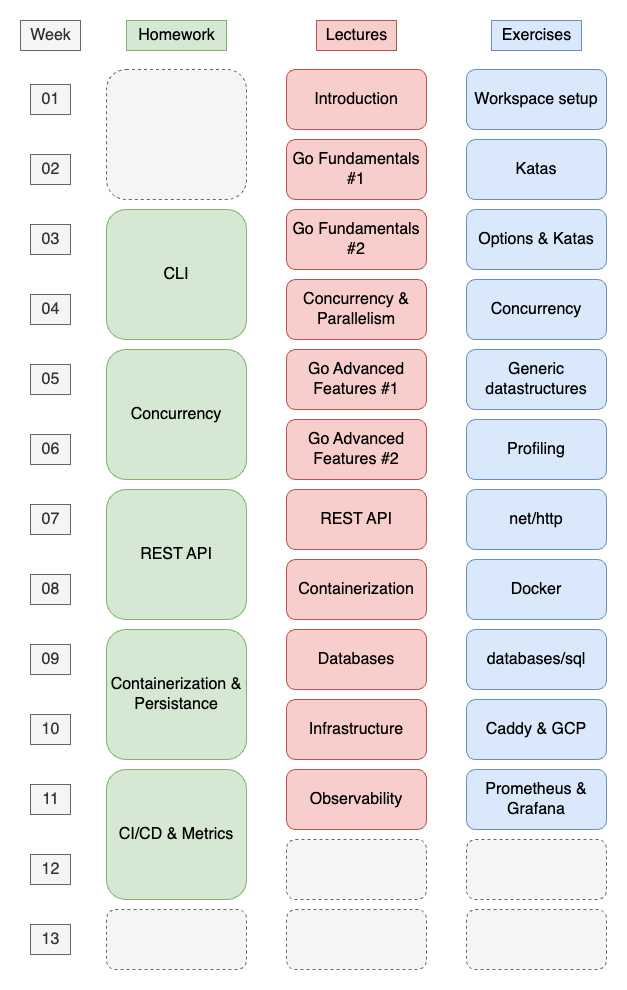
\includegraphics[width=11cm]{figures/schedule.png}
    \caption{Outline of the course.}
    \label{schedule-outline}
\end{figure}

\subsection{Lectures}

The first six lessons are adaptations of the original Red Hat Go Course slides, which underwent major changes and restructuring. The changes were made to make the taught topics more cohesive and easier to follow, as some of the code samples were unnecessarily long or complex. Several lessons, specifically those on REST API and Concurrency, presented outdated principles that warranted updating. Multiple lectures, such as Math \& Go or Python \& Go, were removed altogether as I did not deem them important.

The last five lectures are completely new and extend the course with numerous technologies and third-party libraries. The original course focused solely on using the standard library. Some of the parts of the standard library, notably the default HTTP web router, are generally not leveraged in practice\footnote{Although this might change as it was extended in the Go version 1.22 release.}. The new lectures focus more on practical usage; therefore, they are not limited in this way.

All of the lectures are estimated to take around eighty to ninety minutes. The lectures should be followed by starting the implementation of the exercises further described in \cref{exercises}.

\subsubsection{Tooling}

I considered multiple tools for creating the lecture slides. For numerous reasons, I reviewed only markdown-oriented technologies. The major reason was that all materials were intended to be versioned using git, so a plain-text solution was necessary. This was done to ease collaboration with potential open-source contributors, which can further extend the course or fix any existing mistakes. The course also includes code exercises and examples that needed to be versioned, so merging all of these materials under a single GitHub organization seemed the most reasonable.

The original Red Hat Go course used the Go Present tool\cite{go-present}. This solution, created by the Go team, implements an exceptional feature: it can run the Go code in your slides and immediately present the output. For this reason, I decided to continue using it for the new lectures, as any other markdown-styled solution did not offer any similar viable alternative.

I also considered Marp\cite{marp} as the runner-up. This tool is used throughout the PV281: Rust course previously mentioned in the \cref{rust-course}. Compared to the Go Present tool, the main benefits include much better formatting capabilities, the possibility of exporting slides to multiple data formats like PDF or HTML, and a more straightforward syntax.

\subsection{Exercises}\label{exercises}

The exercises are designed to be complementary assignments to lectures. The general feedback on the first course run, as discussed in the \cref{additional-exercises}, was a lack of hands-on experience. These exercises were designed to compensate for that. They are, by no means, an equivalent substitute for traditional standard seminars. The students are expected to spend only up to thirty minutes solving them.

Each lecture is paired with a single exercise that can, in some cases, be split into up to two tasks. Both of these, in some way, relate to the topics covered in the lecture.

The exercises are not intended to be graded. However, they can be reviewed or evaluated as they can provide useful on-site insight into the student's understanding of the covered topic, which can be reflected later. These exercises should also serve as the ground for answering potential follow-up questions on the lecture topics.

It is worth noting that the exercises are not necessarily intended to be completely finished. They are expected to take up around twenty to thirty minutes. That amount of time will usually not be left after giving the lecture. As noted previously, some exercises comprise multiple tasks; in such cases, you can prioritize which one you deem more important and instead do just the single task.

\subsection{Homework}

The homework assignments are a form of individual work. Their goal is to prepare students for their final projects. The first two homework assignments are independent, while the last three depend on each other and demonstrate building an application from the ground up.

The students start by forking the original homework assignment repository, making it private, and adding their tutors to the repository. The assignments are then submitted as a pull request into these private repositories, where they will be reviewed.

Starting from the third week, the assignments are published with a ten-day deadline followed by a four-day review period. The review period is designed to give students feedback that they will later incorporate into their solutions.

No sample solutions for the homework assignments currently exist. However, they are planned to be implemented before the commencement of the semester to further verify the assignment's clarity and overall feasibility.

\subsection{Projects}

The projects are the final part of the course. They are estimated to take fifty to sixty hours\footnote{This requirement will need to be decreased to twenty-five to thirty hours if the course is to be run under the Domain-specific Development course. This is done solely to match the course extent.} for each student. The size of the projects should approximately match that estimation.

To initiate the projects, students are presented with a set of technologies or libraries they can leverage in their project implementations in a bonus lecture described thoroughly in \cref{lecture-projects}. This lecture subordinately serves as a form of motivation.

The general incentive is to make students come up with their own projects. Therefore, no "official" project assignments will be published. This was deeply considered as it may demotivate some students in the final part of the semester. However, I believe that the exploratory bonus lecture is sufficient for driving the students' projects even without predefined assignments.

No matter the choice of project, all of them are finished with a short defense during the examination period. These defenses can be organized either physically or online. Students are expected to give a short presentation and a demonstration. Students should also cover used technologies and libraries and briefly describe their experiences and struggles.

There are two reasonable approaches on how to review the projects.
\begin{itemize}
    \item The first one is to review the projects before the defense and confront the student during the defense. This allows confronting the students and having a discussion to reflect on the student's solutions and their potential mistakes. On the other hand, it slightly prohibits public defenses in the presence of other students.
    \item The second one is to review the projects after the defense. This permits the creation of public sessions that multiple students can attend at once, as no personal questions are raised. On the other hand, it makes the follow-up review less personal, and the student cannot be reasonably confronted.
\end{itemize}

There are multiple means of completing the project, each offering a different set of advantages and disadvantages. The course is designed not to be overly restrictive, therefore giving flexibility of choice for the projects.

The project assignment can be fulfilled in three ways:
\begin{itemize}
 \item Implementing a team project.
 \item Implementing a solo project.
 \item Creating an open-source contribution.
\end{itemize}

\subsubsection{Team projects}

The team projects required coordination between the team members; therefore, it simulates practical collaboration the most. However, it restricts students as they have to agree on a single project assignment. 

The students can group into up to four-member teams, but two or three-membered teams are preferred. The size of the projects should be linearly scaled with the number of team members. I do not recommend exceeding these numbers, as it is generally observed that any higher number may negatively affect the teams' performance. It mostly only brings an additional overhead and introduces large project requirements.

When evaluating projects, it should be verified that the work was roughly evenly distributed between the students. As often happens, some students leave most of the work for their team members and only join in on minor tasks, if at all. Such lack of activity should be reflected in the student's evaluation.

It should also be noted that sometimes, a student implements most of the project assignments independently without giving the rest of the team a chance to contribute appropriately. Differentiation between the two cases is merely impossible. The only way is to consult the team members directly, and even then, the active students tend not to report on and abandon their peers.

\subsubsection{Solo projects}

The solo projects give the most flexibility. Students can implement their own assignments without consulting or cooperating with other team members. This, for example, allows them to implement a project they have long thought about but did not find enough time for its realization.

On the other hand, the lack of interaction with peers is also the biggest disadvantage. The goal of these projects should, at least to some extent, be to get students familiar with real-life software project collaboration. Such projects are hardly implemented by solo developers.

Based on the first course run, students opted for this option the most as it is perceived as the path of least resistance. Hence, it should be expected that most projects will be of this kind.

\subsubsection{Open-source contributions}

The open-source contributions are rather experimental. The main motivation behind this variant is to allow students to get involved in the open-source community, give them a guiding hand, and provide feedback during their first steps. 

This path presents several challenges to the students. First, the students must find open-source projects to contribute to. Secondly, they must engage, review current issues, and participate in the discussion and codebase. Lastly, they must implement the changes and get them reviewed and merged.

The pull or merge requests do not have to be merged at the time of the defense, as the tutors cannot guarantee the maintainers' activity. This can be tackled by providing projects maintained by tutors or their colleagues. However, such appropriate "good-first" projects that are simultaneously maintained by the tutors often hardly exist.

The contributions can be split up into multiple pull or merge requests, even to different projects. Therefore, opening a larger pull request and opening multiple smaller ones are both acceptable variants.

The size expectations for the open-source contributions are much lower than those for its project alternatives. Upon its evaluation, the process of searching for an open-source project to contribute to and further involvement in the codebase is considered.

It should be noted that contributing to projects with low activity or without active maintainers should be avoided.

Our faculty does not promote open-source collaboration enough. The faculty's lack of permanent open-source-oriented courses exploring open-source workflow and etiquette can further support this statement. Some efforts to introduce such courses have been made in collaboration with industrial partners in the past few years. These open-source projects also try to push this motion forward.

\section{Comparing with existing courses}\label{reflect-course}

The overall course design was mostly inspired by the existing PV281: Rust course described in \cref{rust-course} and additionally resembles\footnote{The Go course was mostly designed before I had the chance to attend the Java course.} the PA165: Enterprise Java course described in \cref{enterprise-java-course}.

Compared to the PV281: Rust course, the Go course does not cover any client-side development\footnote{This is covered by the HTMX and Tauri lecture in the Rust course.}, and instead solely focuses on the backend development. The Go course also covers containerization and the Docker platform described in \cref{lecture-containers}, which the Rust course did not cover and implicitly expected its knowledge. 

The overall teaching methods are also inspired by the PV281: Rust course with some deviations. Instead of dedicated Rust seminars, the Go course has exercises. Instead of ten iterations\footnote{Small homework tasks, one for each week.}, the Go course has five homework assignments. Lastly, the Go course offers more flexibility of choice as the projects do not have predefined topics as the Rust course dost\footnote{Students can also create their own custom topics after consulting with tutors.} and do not require four-member teams like the Rust course.

Compared to the PA165: Enterprise Java course, the Java course covers OAuth2, microservices, and various methods of authentication and messaging, while the Go course covers infrastructure, containerization, and Docker in greater depth. Otherwise, the scope of the Go and Java courses is similar.

\section{Reflecting feedback}\label{reflect-feedback}

The lectures now also explore the discussed topics in \cref{general-feedback} in greater detail. Some of them, like the Docker or the structuring of Go projects, were previously not covered at all.

The new outline also raised some concerns in \cref{sneakpeek} regarding the scope of the course. 

The first was that the scope of the course got rather large, with topics not directly related to Go. As was previously declared, the goal of the course is to equip its students with the knowledge required to build production Go applications. Although some of the topics do not necessarily relate to Go, namely Observability, Infrastructure, or Containers lectures, they are applied to the Go environment and demonstrate the process that is involved when implementing, deploying, and maintaining such production applications. For this reason, I decided that they were a good addition to the course's content. However, it is worth noting that these topics could be later extracted to a separate course as described in the \cref{devops-overlap}. Currently, there is no such opportunity to do this so for the time being, these topics will be covered in the Go course directly.

The second concern is that the course will become time-consuming with the addition of homework assignments combined with the projects. The reality is that the course's first run was overcredited as we did not require any attendance, and the only required output was the completion of the project. The parent course, Domain-driven Development, under which the Go course runs, currently has an extent of three European Credit Transfer and Accumulation System (ECTS) credits. Adding these additional homework assignments will align the extent of the course more with its parent course.

\section{Evaluation}

Students can acquire up to one hundred points in total. From these one hundred points, a minimum of seventy has to be acquired. The first half of these points can be received by completing the homework assignments, while the second half is obtained by completing the project.

There is a common requirement for all of the graded tasks. This requirement is that all Go code is written idiomatically, avoiding common mistakes and misconceptions.

\subsection{Homework}

The points for homework assignments are not distributed evenly as the two first homework are smaller in size and scope. Therefore, the first two homework assignments are graded by up to seven points each, while the last three are twelve points each. Each homework defines a set of requirements and expectations.

\subsection{Projects}

Defining precise grading criteria for projects is slightly problematic as they can vary heavily in scope and focus. However, some basic common criteria can be declared and are further described in this section. None of the following requirements apply to the open-source contribution projects, as they simply do not make sense. \\

\noindent
All projects should:
\begin{itemize}
    \item follow the standard structure as specified by the de facto Go project layout standard\cite{go-project-layout}.
    \item include a continuous integration pipeline that lints, formats, builds, and tests the projects and a continuous delivery pipeline that publishes a docker image to a public repository of any choice.
    \item implement minimal happy-path test cases using the Go testing suite.
    \item should include single or multiple scenarios that demonstrate its usage and that can be executed to verify basic functionality.
\end{itemize}

\noindent
Bonus points can be gained by performing additional actions such as deploying the application, instrumenting the application with telemetry, setting up monitoring, creating an OpenAPI specification, heavily testing the application, etc.

\subsection{Bonus points}

Additional bonus points can be acquired by being active during lectures and exercises or submitting exceptional solutions for homework and projects. This rewards engaged students and promotes further activity during the lectures.

\section{Limitations}

This section describes some possible inefficiencies that were later perceived but were currently not incorporated into the course. Some of these will be considered as additions to the course in the future.

\subsection{Auth}

The course does not cover authorization or authentication in any way. It is up to debate if the course should cover this topic and, if so, to what extent. I believe that education in this regard, especially with practical application, is insufficient at our faculty. A dedicated course tackling topics like JSON Web Tokens (JWT)\cite{jwt}, Cookies, and OAuth2\cite{oauth2} and their usage should exist instead. None of these concepts are currently covered in depth by any course.

\subsection{APIs}

The course currently covers designing and implementing REST APIs. This is still the standard for most service communication. However, during the past decade, multiple other approaches emerged that are often incorporated into systems in practice, notably gRPC\cite{grpc} and GraphQL\cite{graphql}. These were not added to the course but could be considered in the future as they are highly related to backend development.

\subsection{Event-driven communication}\label{edc}

Event-driven communication solves multiple problems imposed by today's world of distributed architectures. Giving a basic overview of how these systems work and how to integrate such systems should be considered in the future. Notable Go projects that exist regarding this topic are the NATS\cite{nats} message broker, the event-driven commutation library Watermill\cite{watermill}, and the messaging server Cetrinfugo\cite{centrifugo}.

\subsection{DevOps/Ops overlap}\label{devops-overlap}

Some of the lectures, namely Containerization, Infrastructure, and Observability (all covered in depth in \cref{lecture-containers,lecture-infrastructure,lecture-observability} respectively) overlap with the DevOps/Ops field. Although the lectures provide Go examples and try to apply the general knowledge to Go, these topics are not, in broad, Go specific and could be extracted to an additional course in the future. This would free up space for other topics, such as those previously mentioned. However, no such course currently exists.

\section{Licensing}

The original course is open-sourced under the Creative Commons Attribution-ShareAlike (CC BY-SA 4.0 Deed) license\footnote{\url{https://creativecommons.org/licenses/by-sa/4.0/}}
, and as it is a share-alike license, the new course had to respect it. There was an option to migrate to the GPLv3 license\footnote{\url{https://www.gnu.org/licenses/gpl-3.0.en.html}}
, which is compatible, but in the end, the Creative Commons license was preferred.

The original idea was to keep the new course open-sourced either way, so reusing and adapting the existing course was not a deterrent. The motivation behind this was to keep the course in the public space. Anyone who would like to remix or reuse the course would be free to do so. There is no reason to keep anyone from using any of its materials, even for those with commercial intentions.

\chapter{Course content}\label{chapter-content}

The content is described in the same order as it is presented to students throughout the semester.

All of the lectures start by briefly explaining their content, followed by the expected knowledge prior to attending the lecture and the expected knowledge gained following the lecture attendance. A precise lecture outline is then given, followed by a more detailed description of the lecture's content.

\section{Lecture 00: The course}

This lecture is designed solely to provide elementary information about the course, such as its requirements and outline.

\section{Lecture 01: Introduction}

This lecture introduces the Go programming language and explores its current state and strong points. It also goes over the installation of Go and basic CLI usage and demonstrates Go basics using a Hello World example.

Students are expected to understand the current state of the language and be able to run Go code using the Go executable. No prior knowledge is expected.

\subsubsection{Outline}

\begin{itemize}
    \item Introduction to Go (Origins, Characteristics \& Comparisons, Motivation)
    \item IDEs \& editors
    \item Installing Go
    \item Running Go (Go executable, Modules, Packages, Hello World)
\end{itemize}

\subsubsection{Content}

The first section explores the Go's history and the motivation behind its creation. It also compares it to other related languages and showcases its common use cases in practice.

The second section shows a list of recommended code editors and IDEs that support the Go programming language.

The third section guides the students through the installation of the Go toolkit. It covers both the original Go installation guide and commands for the most commonly used package managers.

The last section delves into the Go itself and describes the Go CLI and all of its commands. It introduces the concepts of packages and modules and shows basic project setup and commonly used layout standards. This section finishes off with running a simple Hello World application.

\subsection{Exercise 01}

The first exercise guides students through setting up a working environment on their machines. Students will install Go itself as well as set-up all relevant environmental variables. Finally, they will practice a basic usage of Go CLI through commonly used commands.

\section{Lecture 02: Fundamentals \#1}

This lecture starts with exploring the core fundamentals of Go. It delves into topics like data types, functions, user-defined data types, and pointers.

Students will be conscious of all the basic data types Go provides and all possible control flow keywords and their semantics. They will be able to write functions, define their own data types, and understand and appropriately use pointers throughout their code.

\subsubsection{Outline}

\begin{itemize}
    \item Types
    \item Variables
    \item Control flow
    \item Functions
    \item User-defined data types
    \item Pointers
\end{itemize}

\subsubsection{Content}

The first section starts with the core fundamental knowledge of basic data types and their default values. These include all numeric variants and their aliases, strings and their encodings, and booleans.

The second section describes all possible declarations of variables and their uses. It goes over their differences and implications and inspects the shadowing concepts.

All control flow variants are then introduced in the third section. It maps all of the keywords with example usage and semantics.

The fourth section introduces functions and declarations. It describes both named and anonymized functions, higher-order functions, or closures. It dedicates multiple slides to the defer keyword, which is extremely useful when freeing resources.

Custom structures and type aliasing are introduced in the fifth section. As Go itself provides no support for enumeration types, an example workaround is provided as it is commonly used in Go. Concepts like anonymous structures and structure embedding are also introduced.

The last section is dedicated to pointers. It shows their basic usage, like referencing and dereferencing, and their interoperation with editable structures as method receivers.

\subsection{Exercise 02}

This exercise lets students solve multiple katas that show commonly made mistakes. These katas all cover topics discussed throughout the lecture.

\section{Lecture 03: Fundamentals \#2}

This lecture continues with the introduction to the fundamentals of Go. This one covers more interesting topics like errors, interfaces, and collections than the previous lecture.

Following this lecture, students will be able to understand the basics of error handling in Go. They will also be able to describe how interfaces are implemented, and they will be able to write idiomatic code using and iterating over the two common collection types, slices, and maps.

\subsubsection{Outline}

\begin{itemize}
    \item Interfaces
    \item Errors
    \item Arrays
    \item Slices
    \item Maps
    \item Range
\end{itemize}

\subsubsection{Content}

The lectures start off with interfaces and their underlying implementations in Go. It also depicts some of the characteristics like implicit satisfying instead of explicit implementation or introduces the empty interface.

The second section follows up on interfaces with the introduction of errors. The section is dedicated to handling error values and their creation, either as in-lined, sentinel, or completely custom errors with additional metadata.

Arrays are introduced in the third section. These are mostly used just as a building block for slices which are explored next.

Slices are introduced next as the dynamic list type in the fourth section. The section further describes the slice's implementation and its implications.

The fifth section inspects the hash-map data structure native to Go. It goes over all of the common operations that can be performed on the map data type and also showcases how it can be used to implement a set. 

The last section covers the range of keywords commonly used to iterate over collection items.

\subsection{Exercise 03}

This exercise is split into two tasks:
\begin{itemize}
    \item This first task, like in the previous exercise, lets students also solve multiple katas that show commonly made mistakes.
    \item The second task explores the options builder pattern commonly used in Go. This pattern is an alternative to the traditional builder pattern and is more idiomatic as it is less verbose and provides more flexibility.
\end{itemize}

\section{Lecture 04: Concurrency \& Parallelism}

The lecture explores Go's concurrency model and dives into all of the synchronization primitives and principles commonly used in idiomatic Go code when building concurrent applications.

After attending this lecture, students will be able to understand the concept of goroutines and Go's runtime model. They will also be able to write concurrent applications leveraging all of the possible synchronization primitives. It is suggested that the students have some conception of concurrency and knowledge of synchronization primitives.

\subsubsection{Outline}

\begin{itemize}
    \item Goroutines
    \item Runtime
    \item Channels
    \item Select
    \item Packages
\end{itemize}

\subsubsection{Content}

The lecture starts with exploring the differences between concurrency and parallelism as shown in \cref{fig:con-vs-par} and is followed by an introduction to the concept of goroutines. This knowledge is further built on in the second section, where Go's runtime model is described. One such state of the runtime environment can be viewed in \cref{fig:runtime}.

\begin{figure}[H]
    \centering
    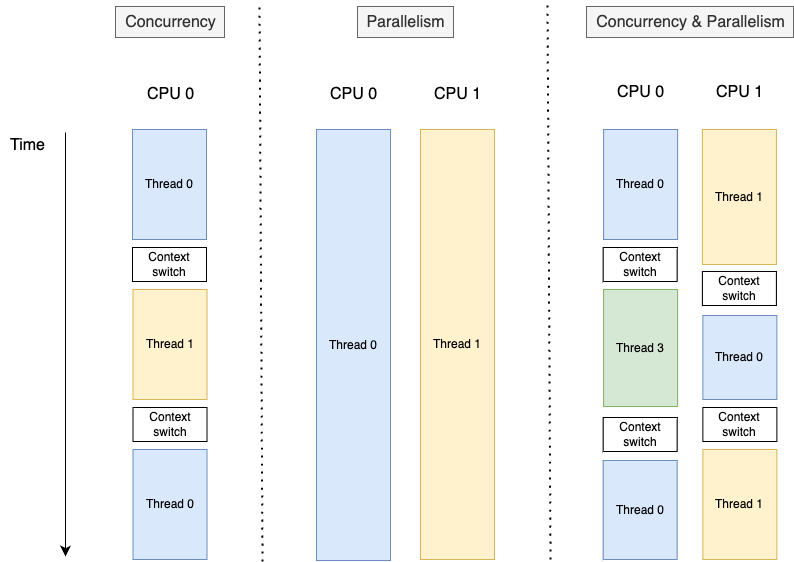
\includegraphics[width=12cm]{figures/concurrency-parallelism.png}
    \caption{Differences between concurrency and parallelism}
    \label{fig:con-vs-par}
\end{figure}

\begin{figure}[H]
    \centering
    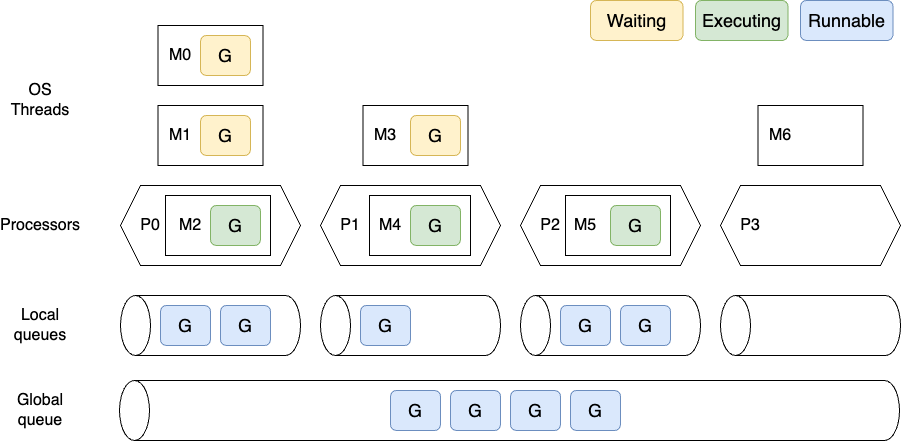
\includegraphics[width=12cm]{figures/scheduling.png}
    \caption{Possible runtime state.}
    \label{fig:runtime}
\end{figure}

The third section introduces the concept of channels as a means of communication for concurrent processes. To better image some of the most common interactions and edge cases, multiple diagrams were created, such as the one in \cref{fig:goroutine-interactions}. The channels section also discussed various patterns commonly used in concurrent systems like the ones depicted in \cref{fig:fanin,fig:fanout}.

\begin{figure}[H]
    \centering
    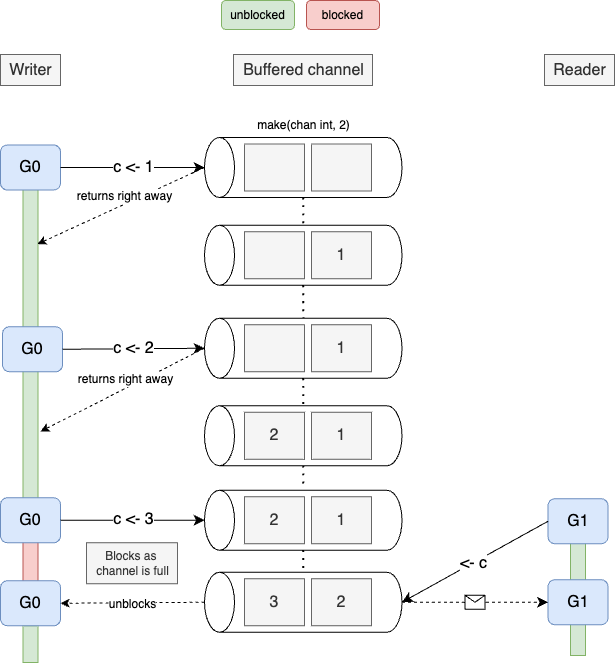
\includegraphics[width=12cm]{figures/buffered-full.png}
    \caption{Interaction between two goroutines interaction via a buffered channel.}
    \label{fig:goroutine-interactions}
\end{figure}

\begin{figure}[H]
    \centering
    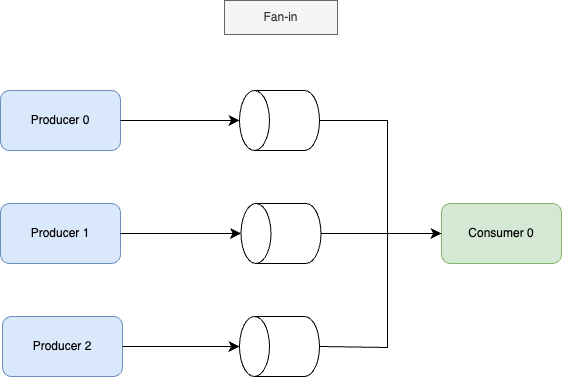
\includegraphics[width=12cm]{figures/fanin.png}
    \caption{Diagram of the fan-in pattern.}
    \label{fig:fanin}
\end{figure}

\begin{figure}[H]
    \centering
    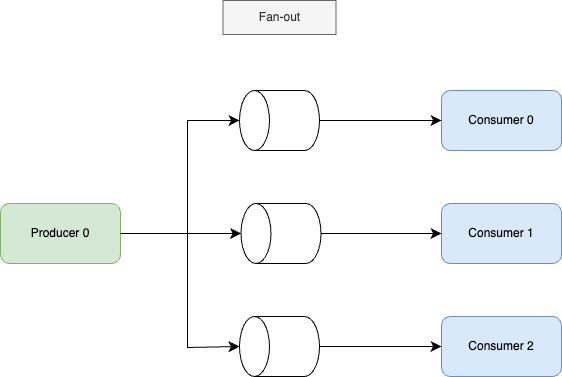
\includegraphics[width=12cm]{figures/fanout.png}
    \caption{Diagram of the fan-out pattern.}
    \label{fig:fanout}
\end{figure}

The last section mostly covers the sync and atomic packages that provide synchronization primitives, such as mutexes, conditional variables or wait groups, and atomic data types.

\subsection{Exercise 04}

In this exercise, students are guided through an implementation of a producer-consumer problem in a service modeling invoice data messaging. The students will need to leverage the knowledge of all of the previously discussed topics like goroutines, contexts, and synchronization primitives. They are then further guided to optimize the application and implement a graceful shutdown for the service.

\section{Lecture 05: Advanced \#1}

This lecture starts the exploration of advanced Go topics. The lecture begins with generics that were added to Go in version 1.18, followed by an overview of the majority of the commonly used standard library packages and finishes with the Go built-in testing framework.

Students will be able to implement all kinds of generic data types, test their applications with various types of tests, and use all of the described tools and packages. No prior knowledge is expected.

\subsubsection{Outline}

\begin{itemize}
    \item Generics
    \item Packages
    \item Testing
\end{itemize}

\subsubsection{Content}

The first section explores the history of generics in Go and how generic data types were implemented prior to their addition. It also explores some of their limitations and showcases possible use cases with the implementations of the map and filter functions.

In the second section, the lecture covers all interesting standard library packages that are often used in practice. These mostly include libraries for manipulating collections like maps and slices, libraries for interacting with the operating system and logging libraries.

Lastly, the lecture describes the different types of tests and testing models as shown in \cref{fig:testing-models} and further continues to explore Go's testing toolchain. Apart from standard testing itself, it also covers fuzzing, which the testing framework supports. Finally, the section is finished with an overview of third party testing libraries that provide more high-level tooling or allow the generating of various types of fakes like stubs of mocks.

\begin{figure}[H]
    \centering
    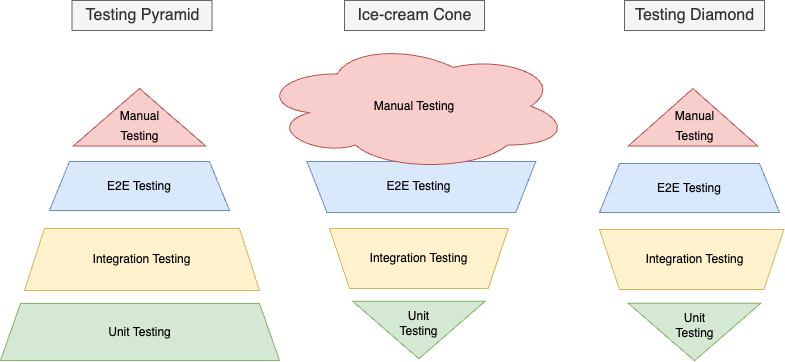
\includegraphics[width=12cm]{figures/pyramids.png}
    \caption{Testing models.}
    \label{fig:testing-models}
\end{figure}

\subsection{Exercise 05}

This exercise lets students implement a generic data structure of their choice, followed by the creation of multiple unit tests using the Go test suite. It also guides the student through creating a coverage profile and how it can be inspected using the go cover tool.

\section{Homework 01}

\section{Lecture 06: Advanced \#2}

This lecture introduces some of the additional advanced topics present in Go. It mainly focuses on performance and optimizations but also covers some of the additional topics like CGo, Unsafe, or Reflection, which could not be included in any other lecture as it either did not make sense or there was simply no space left.

Students will be able to understand common limitations regarding various data types and references and will be able to profile and optimize Go applications after completing this lecture. No prior knowledge is expected.

\subsubsection{Outline}

\begin{itemize}
    \item Benchmarks
    \item Profiling
    \item Optimizations (References \& Values, Maps, Slices, Loops, Strings)
    \item CGo
    \item Unsafe
    \item Reflection
\end{itemize}

\subsubsection{Content}

The lecture starts with introducing the benchmarking tooling in Go. This topic is similar to the testing presented as the last topic in the previous lecture. This was intentionally done to connect these two lectures, giving them a more natural transition.

Profiling go applications is then explored in the second section. The pprof profiling tool is introduced and a description is given about the various types of profiles and all methods for retrieving them.

The third section goes over optimizations commonly done in go and some common mistakes with specific data types that often cause low performance or high memory consumption.

The fourth section introduces CGo as a Foreign Function Interface (FFI) to the C programming language, which Go directly supports in the standard library.

The last two sections cover two standard library packages that leverage reflection, which allows one to examine types at runtime, or the unsafe package, which works around the Go's type system rules and allows such things as manipulating pointers directly.

\subsection{Exercise 06}

This exercise presents students with a webserver that endlessly consumes memory resources. The students then must use the pprof profiling tool to examine the application's performance. They have to both generate the performance profiles using the exposed HTTP endpoints and then visualize them using the appropriate graphs.

\section{Lecture 07: REST APIs}

Starting from this lecture, all of the materials are completely new additions to the course. It is worth noting that the previous course did cover HTTP routing in one of its lectures, but it was outdated, and the new course does not build on top of those materials.

This lecture is dedicated to REST API design and to implementing such APIs in Go. The lecture covers the common fundamentals required to implement such APIs while also covering Go specifics and related technologies. 

Following this lecture, students will be able to design and implement REST APIs using various Hypertext Transfer Protocol (HTTP) frameworks and routers. Only the fundamental knowledge of networking is expected.

\subsubsection{Outline}

\begin{itemize}
    \item JSON
    \item HTTP
    \item REST API
    \item Go \& HTTP (Standard library, Third-party libraries, Testing webservers)
    \item OpenAPI
    \item Templating
\end{itemize}

\subsubsection{Content}

In the first three sections, the lecture briefly goes over the fundamentals like JavaScript Object Notation (JSON), which represents a commonly used data format for data interchange, the HTTP protocol used for transmitting the data, and REST API principles.

The next section is dedicated to HTTP and its specifics in Go. It provides an overview of the most up-to-date and used routers and frameworks, highlighting both the advantages and disadvantages. A short part is also dedicated to testing HTTP servers and clients using Go's standard library packages.

The OpenAPI specification is described as the goto schema definition standard for REST APIs in the second to last section. Multiple libraries that use the specification to create mocks or generate server or client code are also mentioned.

The last section explores the Go's built-in templating engine and showcases its usage. It is explored in this lecture as it can often be used to serve dynamic data over the REST API.

\subsection{Exercise 07}\label{exercise-07}

This exercise starts with implementing an application that is further used in exercises described in \cref{exercise-08,exercise-09,exercise-11}. The application is a simple Todo Create-Read-Update-Remove (CRUD) app with no complex business logic. The OpenAPI\cite{open-api} specification describes the application's API that the students will implement in this exercise.

\section{Homework 02}

\section{Lecture 08: Containers}\label{lecture-containers}

This lecture introduces containerization technology with a focus on practical usage. This knowledge is further required in the following lectures presented in \cref{lecture-databases,lecture-infrastructure,lecture-observability} and as it is currently not covered to the required extent as presented in \cref{code-quality-and-management}, it was incorporated into the course itself.

After the lecture, students will be able to containerize their applications and run their applications and their dependencies using container images. They are only expected to have a basic understanding of virtualization before the lecture.

\subsubsection{Outline}

\begin{itemize}
    \item Containers
    \item Docker (Desktop, Hub, Build, Compose)
    \item Podman
    \item Testcontainers
    \item Kubernetes
\end{itemize}

\subsubsection{Content}

The lecture starts by introducing containerization as a concept while comparing it to virtual machines. This section also provides motivation for using containers and briefly covers the Open Container Initiative (OCI) standards.

The second and most extensive section explores the Docker\cite{docker} platform in-depth. It provides information regarding its history, flows as depicted in \cref{fig:docker}, architecture, and maps all related tools. Most of the time is spent on using the CLI, Dockerfile, and Compose tools. Lastly, a Podman\cite{podman} is mentioned in the third section as an open-source alternative to Docker.

The fourth section covers Testcontainers\cite{testcontainers} as a tool that simplifies the testing process by running dependencies directly in code.

Lastly, the lecture briefly inspects the Kubernetes\cite{kubernetes} platform that further builds on the containerization technology and solves numerous problems that are often faced when building distributed systems, such as horizontal scaling and fault tolerance. This section is not meant to provide thorough insight but to give a broad overview of how Kubernetes works and what it can be used for.

\begin{figure}[H]
    \centering
    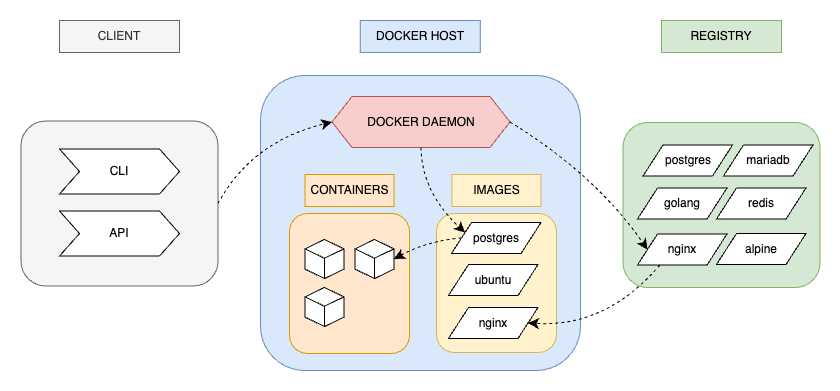
\includegraphics[width=12cm]{figures/docker.png}
    \caption{The Docker flow.}
    \label{fig:docker}
\end{figure}

\subsection{Exercise 08}\label{exercise-08}

During the exercise, students will containerize the Todo application they started with in the previous exercise in \cref{exercise-07}. The exercise is split into two steps. First, the students will create a custom container image using the Dockerfile, which they will then use in Docker Compose.

\section{Lecture 09: Databases}\label{lecture-databases}

This lecture focuses on Relational Database Management Systems (RDBMSs) and their integration with Go applications. The main goal of this lecture is to introduce the various approaches currently viable in the Go ecosystem, from low-level libraries to Object-relational Mapping (ORMs).

As the output knowledge, students will be capable of implementing persistent Go applications while levering RDBMSs. Students are only expected to be proficient in using the Structured Query Language (SQL).

\subsubsection{Outline}

\begin{itemize}
    \item SQL
    \item RDBMSs
    \item Database migrations
    \item Go \& SQL (sql, sqlx, sqlc, GORM)
\end{itemize}

\subsubsection{Content}

The first two sections of the lecture give a brief refresher on SQL and RDBMS. It gives a short overview of the most popular RDBMSs and their key points.

The third section introduces database migrations and their various aspects and challenges. It covers multiple database migration tools and showcases usage via both CLI and in-code.

Lastly, the fourth and biggest section discusses multiple approaches to integrating database access to applications leveraging modern Go libraries. It starts by covering the
support the standard library provides and introduces compatible database drivers. As the standard library defines rather low-level interfaces, multiple libraries try to compensate for this; the most notable is sqlx\cite{sqlx}, which is covered next. It provides more high-level functions that make writing the code less verbose. Thirdly, the sqlc\cite{sqlc} library is showcased as an interesting and untraditional approach as it works by \enquote{compiling} the SQL queries and generating native Go code. The last presented approach is the GORM\cite{gorm} library, which represents Go's most commonly used ORM.

\subsection{Exercise 09}\label{exercise-09}

The exercise builds upon the Todo application started in the previous exercise presented in \cref{exercise-07}. The application in the assignment currently uses an in-memory repository. The goal of the exercise is to extend the existing Docker compose file with a PostgreSQL\cite{postgres} database and rewrite the repository to persist its data using the database instance.

\section{Homework 03}

\section{Lecture 10: Infrastructure}\label{lecture-infrastructure}

The motivation behind this lecture is to give students an insight into the continuous integration and continuous deployment/delivery (CI/CD) process and how this practice can be applied in the context of Go projects. The second goal is to give students a basic knowledge of how such projects can be deployed and maintained.

After attending the lecture, students will be able to set up a basic CI/CD pipeline, provision infrastructure using the Google Cloud Platform, and deploy simple applications. The students are expected to understand basic software engineering practices and elementary networking.

\subsubsection{Outline}

\begin{itemize}
    \item Linters
    \item CI/CD (GitLab CI/CD, GitHub Actions)
    \item Infrastructure
    \item Cloud (Google Cloud Platform)
\end{itemize}

\subsubsection{Content}

The first section covers linters and expands on the knowledge acquired in the introductory lesson, where the built-in go-vet linter was introduced. Most of this section is dedicated to the golangci-lint tool, a linter aggregator incorporated in many projects and is the most complex tool today. Together with formatters, these tools are necessary in the continuous integration process introduced in the following section.

The second section introduces the CI/CD process as depicted in the \cref{fig:cicd}. The primary goal of this section is to provide students with the knowledge to implement the CI/CD pipeline using both GitLab CI/CD\cite{gitlab-cicd} and GitHub Actions\cite{github-actions}.

As the faculty operates a self-hosted GitLab instance, almost all of the git-related work is done using GitLab. Consequently, most students do not interact with GitHub throughout their studies. The secondary goal of this chapter is to familiarize students with GitHub so they can join the open-source community, as most open-source software is developed on the GitHub platform.

\begin{figure}[H]
    \centering
    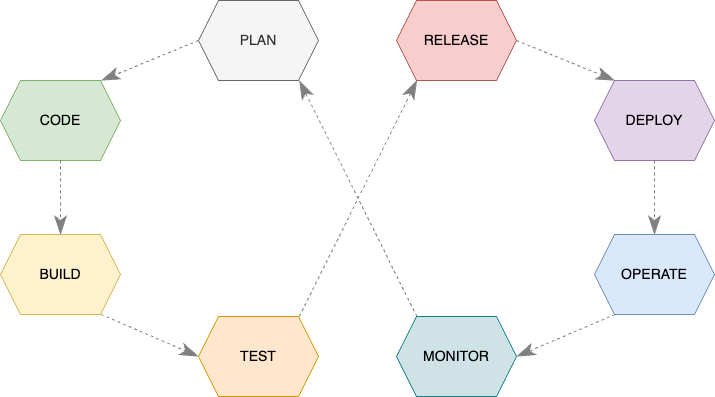
\includegraphics[width=12cm]{figures/cicd.png}
    \caption{CI/CD pipeline.}
    \label{fig:cicd}
\end{figure}

The third section gives an introduction to infrastructure design. Introduces basic concepts such as proxying, load balancing, and application scaling and goes through multiple examples, one of which is depicted in the \cref{fig:infra}. Two related technologies are introduced to leverage these concepts, namely Traefik Proxy\cite{traefik} and Caddy\cite{caddy}. This section aims to give students a basic understanding of how to provision basic infrastructure and tackle basic infrastructure design problems such as fault tolerance, scaling, or encryption.

\begin{figure}[H]
    \centering
    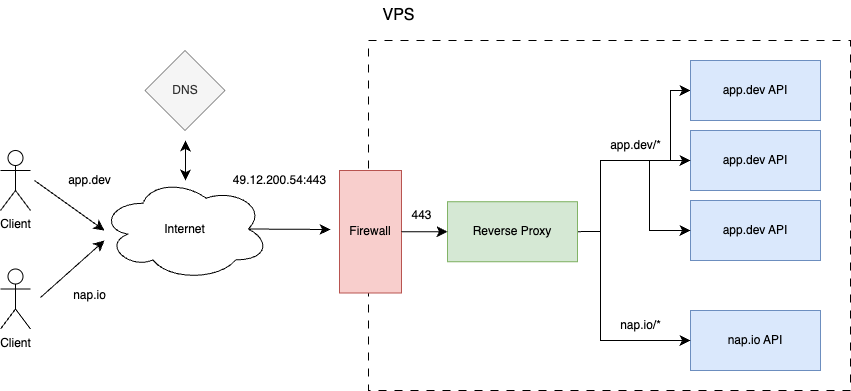
\includegraphics[width=12cm]{figures/infrastructure.png}
    \caption{One of the infrastructure example diagrams.}
    \label{fig:infra}
\end{figure}

The last section introduces all major cloud providers (Amazon, Microsoft, and Google) and further delves into Google Cloud Platform (GCP)\cite{gcp}. As Google offers free credits thanks to the faculty program\cite{gcp-faculty}, it is a great opportunity for students to get their hands on operating cloud infrastructure. A set of basic services that GCP offers are introduced so students can leverage these in their final projects.

\subsection{Exercise 10}\label{exercise-10}

The exercise comprises two tasks. The second task is more of a demo in which the tutor will guide the students through the GCP Console.

As students generally have a basic understanding of CI, thanks to their previous experiences, it is not practiced at the seminar. Instead, the seminar time is given to the GCP. The goal of the demo/exercise is to get students familiar with the GCP so they can provision their own infrastructure. \\

\noindent
Tasks:
\begin{itemize}
    \item The first task involves setting up a Caddy server instance as a reverse proxy/load balancing multiple ping-pong service instances. You can learn more about the ping-ping application in the \cref{apendix-materials}.
    \item The second task involves setting up an automatic build and deployment using Cloud Run\cite{gcp-cloud-run}, provisioning a Compute Engine\cite{gcp-cloud-compute} virtual machine, and a Cloud SQL SQL\cite{gcp-cloud-sql} server that can later be used for the student's projects.
\end{itemize}
    
\section{Lecture 11: Observability}\label{lecture-observability}

This lecture delves into the topic of observability. The lecture covers all major types of telemetry signals, namely metrics, logs, and traces. Each signal is briefly introduced, after which specific state-of-the-art\footnote{Many alternative technologies to the ones provided exist. The selection was made based on a general prevalence and on the fact that they are open-source and implemented in Go.}
technologies are introduced. In the last part, the OpenTelemetry\cite{open-telemetry} project is introduced.

Following the lecture, students should be able to set up the introduced technologies, instrument their applications with basic telemetry, and monitor their applications' health. No previous knowledge regarding observability is required.

\subsubsection{Outline}

\begin{itemize}
    \item Health
    \item Metrics (Prometheus, Grafana)
    \item Logs (Loggers, Loki)
    \item Traces (Jaeger)
    \item OpenTelemetry
\end{itemize}

\subsubsection{Content}

The lecture starts off with an introduction to concepts such as health and heartbeat and shows how to export application status.

The next section covers the first of the three major signal - metrics. A brief explanation with multiple metric examples is given. The spotlight is then transferred to the Prometheus project.

Prometheus\cite{prometheus} is undeniably the leading project that revolves around retrieving, storing, and evaluating metrics. The Prometheus format is supported by multiple third-party tools. The section introduces the Prometheus format and the various metric types it supports.

Lastly, this section introduces Grafana\cite{grafana} as the project of choice for visualizing metrics. The slides refer to the Granafa sandbox\footnote{ \url{https://play.grafana.org/d/000000012/grafana-play-home}}
that can be explored during the lecture shortly.

The second signal to cover is logs. This section puts logs into context and introduces additional structured logging libraries that offer additional features and focus more on performance compared to standard library packages.
The technology of choice for logs is Loki\cite{loki}. Created by the Grafana Labs, it is a log aggregation system heavily inspired by Prometheus. The lecture covers the basic setup and summarizes possible clients and agents that can be used to retrieve the logs.

The final presented signal is traces. As traces are the most complex of all the mentioned telemetry types, a more thorough introduction is given. Then, a transition to Jager\cite{jaeger} is made.

Like with Loki, the slides introduce Jaeger architecture and core concepts. As Jaeger dropped support for all of its previous clients and now only supports OpenTelemetry API and SDK, the instrumentation part is left out and shown in the following section, where OpenTelemetry is explored in-depth.

The OpenTelemetry\cite{open-telemetry}
project is an initiative that has gained much traction in recent years. Backed by the Cloud Native Computing Foundation (CNCF)\cite{cncf},
it is currently the leading project in defining telemetry standards. As of today, all major cloud providers support it. The last section gives insight into the OpenTelemetry Collector and its architecture showcased in \cref{fig:otel}, explains how OpenTelemetry works, and how applications can be instrumented using its Go API and SDK.

\begin{figure}[H]
    \centering
    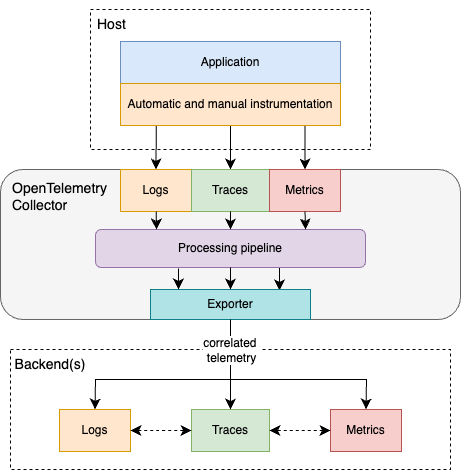
\includegraphics[width=10cm]{figures/opentelemetry-architecture.png}
    \caption{OpenTelemetry architecture inspired by the specification diagrams\cite{open-telemetry-spec}.}
    \label{fig:otel}
\end{figure}

\subsection{Exercise 11}\label{exercise-11}

Similarly to the previous exercise, this one comprises two tasks. The second task is also more of a demo where the students will explore the OpenTelemetry Demo\cite{open-telemetry-demo} with the help of their tutors.

As I deemed metrics the most important to cover, the first task was dedicated to instrumenting and visualizing them. Logs are not really interesting to cover, and traces are rather complex to implement in a limited time span. Instead of trying to instrument an application with all of the related telemetry types, the exercise later moves on to the OpenTelemtry Demo in the second task, which has all of the mentioned things already implemented and better showcases real usage. \\

\noindent
Tasks:
\begin{itemize}
    \item The first task continues with the Todo application that students previously worked on during the exercises described in \cref{exercise-07,exercise-09}. Their objective is to instrument the application with Prometheus metrics and create Grafana dashboards to visualize them.
    \item The second task involves running the OpenTelemetry Demo and interacting with the system. The system consists of multiple microservices implemented in multiple programming languages and instrumented with various types of telemetry while using the OpenTelemetry SDKs. This demo serves as a nice introduction to the OpenTelemetry ecosystem and also includes all of the presented technologies except for Loki, which is replaced with OpenSearch\cite{opensearch}.
\end{itemize}

\section{Homework 04}

\section{Bonus Lecture: Projects} \label{lecture-projects}

The motivation for this lecture is to provide students with an overview of state-of-the-art libraries that can be used in the final Go projects. The technologies are split up into multiple sections depending on their use case.

\subsubsection{Outline}

\begin{itemize}
    \item CLI
    \item TUI
    \item Desktop
    \item Web
    \item Open-source
\end{itemize}

\subsubsection{Content}

The Command Line Interface (CLI) section provides basic information about the most frequently used libraries to implement command-line applications. These libraries include the Cobra\cite{spf13-cobra} and the CLI\cite{urfave-cli}.

The lecture continues by introducing the Bubbletea\cite{charmbracelet-bubbletea} framework and its ecosystem for creating Terminal User Interface (TUI) applications.

The third section introduces possible libraries for implementing desktop applications. The first framework it introduces is Wails\cite{wailsapp-wails}, an alternative to JavaScript Electron \cite{electron-electron}, or Rust Tauri\cite{tauri-apps-tauri} frameworks. The second mentioned library is Fyne\cite{fyne-io-fyne}, which, also from desktop environments, supports the iOS and Android mobile platforms.

The web sections mentions the possibility of creating a web application with a combination of Go backend and an optional frontend technology. The HTMX\cite{bigskysoftware-htmx}, an HTML extension, is mentioned as an alternative to traditional single-page applications (SPAs).

The lecture ends with giving multiple links to resources related to open-source development or possible Go projects.

\chapter{Conclusion}\label{chapter-conclusion}

The goal of this thesis was to design a comprehensive course on Go. The thesis implemented new exercises and homework assignments and revamped the existing Red Hat Go Course lectures while introducing new topics and giving reasoning for the decisions and design changes performed. The course materials created during this thesis form a great basis for the new course which can further be expanded.

\section{Future work}

The course will have to evolve as the language and technologies evolve. I am dedicated to maintaining and developing the course to keep it up-to-date so it can be taught in the future.

The Go course will be run under the Domain-specific Development course the next semester. It could be later extracted into its own separate course to eliminate some of the limitations imposed by running under a parent course, such as the shared extent and intensity.

As discussed in the \cref{devops-overlap}, a new course could also be created in the future to cover some of the topics not necessarily tied with Go. This course could serve as a prerequisite to the Go course and other similar courses in the future.

\printbibliography[heading=bibintoc]

\appendix
\chapter{Course materials}\label{apendix-materials}

All course materials are maintained under the course-go\footnote{\url{https://github.com/course-go}} GitHub organization. To preserve the current state of the materials, all relevant repositories were exported and compressed into an attachment to this thesis. Each top-level directory in the attached archive maps to a GitHub repository. The directories contain versions of materials that existed when submitting this thesis and are most likely out-of-date as you read this text. Inspect the respective GitHub repositories if you want to view the updated version.

The GitHub repositories for respective directories can be found under the following URLs:
\begin{itemize}
    \item lectures\footnote{\url{https://github.com/course-go/lectures}}
    \item exercises\footnote{\url{https://github.com/course-go/exercises}}
    \item homework\footnote{\url{https://github.com/course-go/homework}}
    \item code\footnote{\url{https://github.com/course-go/code}}
    \item course\footnote{\url{https://github.com/course-go/course}}
    \item ping-pong\footnote{\url{https://github.com/course-go/ping-pong}}
\end{itemize}

\section{lectures}

The lectures directory contains all slides and their respective assets (images, code samples, videos, etc.). The supplied README in the directory guides you on how to run the slides.

\section{exercises}

The exercises directory contains all exercises with assignments and related code. Each exercise is in a separate directory containing a README specifying the assignment.

\section{homework}

The homework directory contains all homework assignments. Each homework assignment is located in its respective directory. The assignments are given in the form of a README.

\section{code}

The code directory contains source code that either implements solutions to some of the exercises or implements some form of functionality used throughout the exercises.
\section{course}

The course directory contains information that is the starting point when people want to learn more about the course.
\section{ping-pong}

The ping-pong directory contains a simple REST API project used for teaching deployments and their automation. It is split up from the code project as it simplifies the deployments.

\chapter{Catalog specification}

This chapter specifies the common catalog used to describe courses at Masaryk University.

\subsubsection{Extent and Intensity}

The following expression notes the intensity of lectures, seminars, and homework, plus the type of completion, respectively. \\

\noindent
(1/1/1) + 1 (colloquium)

\subsubsection{Prerequisities}

No hard requirements are enforced. However, students are expected be proficient in using SQL (PB154)\footnote{ \url{https://is.muni.cz/predmet/fi/podzim2023/PB154?lang=en}.}, must possess programming fundamentals (IB111)\footnote{ \url{https://is.muni.cz/predmet/fi/podzim2023/IB111?lang=en}.} and have a basic understanding of networking (PB156)\footnote{\url{https://is.muni.cz/predmet/fi/jaro2024/PB156?lang=en}.} and virtualization (PB152)\footnote{\url{https://is.muni.cz/predmet/fi/jaro2024/PB152?lang=en}.} to the extent of the referenced courses.

\subsubsection{Enrolment limitations}

The course is intended to be run with up to 20 students. It can later be scaled to a higher number, but currently, the intent is to test the new course in practice and interact more with students, which does not scale well and would require opening a second seminar.

\subsubsection{Course objectives}

Students will understand the fundamentals of the Go programming language and its common use cases in practice. They will acquire the required knowledge for entry-level Go developer positions while writing idiomatic Go code, and they will be capable of applying this knowledge to real-life projects.

\subsubsection{Learning outcomes}

Students will be able to:
\begin{itemize}
    \item Write idiomatic Go code.
    \item Understand the Go concurrency model.
    \item Profile and optimize Go applications.
    \item Develop REST API services.
    \item Containerize and deploy their applications.
    \item Implement persistence leveraging SQL databases.
    \item Instrument applications with various types of telemetry.
\end{itemize}

\subsubsection{Syllabus}

\begin{enumerate}
    \item Introduction: (Introduction to Go, IDEs and editors, Installing Go, Running Go)
    \item Fundamentals \#1: (Packages \& Visibility, Variables, Data types, Control flow, Functions, Pointers, User-defined data types)
    \item Fundamentals \#2: (Interfaces, Errors, Arrays, Slices, Maps, Range)
    \item Concurrency \& parallelism: (Goroutines, Runtime, Channels, Select, Related packages)
    \item Advanced \#1: (Generics, Packages, Testing)
    \item Advanced \#2: (Benchmarks, Optimizations, CGo, Unsafe \& Reflect)
    \item REST APIs: (JSON, HTTP, REST API, HTTP package, Routers \& Web frameworks, OpenAPI, Templating)
    \item Containers: (Containerization, Docker, Kubernetes)
    \item Databases: (SQL, RDBMSs, Migrations, SQL, sqlx, sqlc, GORM)
    \item Infrastructure: (CI/CD, Infrastructure, Google Cloud Platform)
    \item Observability: (Health, Logs, Metrics, Traces, OpenTelemetry)
\end{enumerate}

\subsubsection{Literature}

\begin{itemize}
    \item BODNER, Jon. Learning Go. O’Reilly, 2024.\cite{learning-go}
    \item HARSANYI, Teiva. 100 Go Mistakes and How to Avoid Them. Manning Publications, 2022.\cite{100-go-mistakes}
    \item HOLMES, Joel. Shipping Go. Manning Publications, 2023.\cite{shipping-go}
\end{itemize}

\subsubsection{Teaching methods}

In-person lectures with hands-on exercises and reviewed homework assignments and projects.

\subsubsection{Assessment methods}

Multiple homework assignments (fifty points) and a final project (fifty points), including its defense. Seventy out of the one hundred points are required to successfully complete the course.

\end{document}